\chapter{Permutations}
\epigraph[author={Herman Melville},source={Moby Dick}]{I cherish the greatest respect towards everybody’s religious obligations, never mind how comical.}\SubIndex{Melville, Herman}\SubIndex{Moby Dick}
\epigraph[author={Herman Melville},source={Moby Dick}]{Hell is an idea first born on an undigested apple-dumpling.}\SubIndex{Melville, Herman}\SubIndex{Moby Dick}
\section{Transformation groups}
Take a set \(X\), which could be a set of points in the plane, or a set of numbers, or a collection of various geometric figures, or the set of books in a library, or any other set of any sort of things.
A \emph{transformation}\define{transformation} \(f\) of \(X\) associates to each element \(x\) of \(X\) some element \(f(x)\) also from \(X\).
\begin{example}
Take a square \(X\) in the plane, and rotate it around its centre by a right angle.
Each point \(p\) of \(X\) is rotated into some point \(f(p)\).
Note that the centre point of the square is ``fixed'', i.e. rotated into itself.
\end{example}
\begin{example}
Take any set \(X\).
The \emph{identity transformation}\define{transformation!identity}\define{identity transformation} is the transformation that leaves every point of \(X\) where it is: \(f(x)=x\).
\end{example}
\begin{example}
Shuffle a deck of cards.
If \(X\) is the set of cards, the shuffle is a transformation \(f\) of \(X\).
\end{example}
Two maps \(f \colon X \to Y\) and \(g \colon Y \to X\) between sets are \emph{inverses}\define{inverse} if \(f(g(x))=x\) and \(g(f(x))=x\) for any element \(x\) of \(X\).
In other words, \(f \circ g\) and \(g \circ f\) are both the identity transformation.
Recall that a map \(f\) is \emph{invertible}\define{invertible!transformation}\define{transformation!invertible}, also called a \emph{bijection}\define{bijection} or a \emph{permutation}\define{permutation} if it has an inverse.
\begin{problem}{groups:bijection}
A map \(f \colon X \to Y\) of a set \(X\) is \emph{injective}\define{injective} (also called \emph{one-to-one}\define{one-to-one}) if \(f(p)=f(q)\) only when \(p=q\).
It is \emph{surjective}\define{surjective} (also called \emph{onto}\define{onto}) if every element \(y\) of \(Y\) has the form \(y=f(x)\) for some element \(x\) of \(X\).
Prove that a map is a bijection just when it is injective and surjective.
\end{problem}
\begin{problem}{groups:bijection.finite}
Prove that a transformation \(f\) of a \emph{finite} set \(X\) is injective just when it is surjective, and hence just when it is a bijection.
\end{problem}
\begin{answer}{groups:bijection.finite}
Denote by \(\cardinality{S}\) the number of elements in a set \(S\).
We use the basic fact that if \(S \subseteq T\) is a subset of a finite set \(T\), then \(\cardinality{S} \le \cardinality{T}\), with equality just when \(S=T\).
The image of \(f\) is \(f(X) \subseteq X\), equality just when \(f\) is surjective, i.e. just when \(\cardinality{f(X)}=\cardinality{X}\).
Each element maps somewhere, i.e. lies in \(f^{-1}(x)\) for some \(x \in f(X)\):
\[
\cardinality{X} = \sum_{x \in f(X)} \cardinality{f^{-1}\set{x}}
\ge \sum_{x \in f(X)} 1 = \cardinality{f(X)},
\]
with equality, i.e. \(f\) surjective, just when \(f^{-1}\set{x}\) has one element for every \(x \in f(X)\), i.e. just when \(f\) is injective.
\end{answer}
\begin{problem}{groups:transformations.associative}
Prove the \emph{associative law}\define{associative law} for transformations: if \(f,g\) and \(h\) are transformations of a set \(X\), then \((f \circ g) \circ h=f \circ (g \circ h)\).
\end{problem}
\begin{problem}{groups:bijection.inverse}
Prove that a bijection \(f\) has a unique inverse.
\end{problem}
The inverse of a bijection \(f\) is denoted \(f^{-1}\).

A \emph{transformation group}\define{group!transformation}\define{transformation!group} \(G\) on a set \(X\) is a nonempty collection of permutations of \(X\) so that 
\begin{enumerate}
\item 
if \(f\) and \(g\) are in \(G\) then \(f \circ g\) is in \(G\).
\item
if \(f\) is in \(G\) then \(f^{-1}\) is also in \(G\).
\end{enumerate}

\begin{example}
Take \(X\) the Euclidean plane.
Every rotation of the plane around the origin is by some angle, say \(\theta\).
Conversely, every angle \(\theta\) is the angle of some rotation around the origin.
So angles form a transformation group \(G\), the group of rotations of the plane \(X\) around the origin.
\end{example}
\begin{example}
Take \(X\) to be three dimensional Euclidean space.
Take a line \(\ell\) through the origin, with a chosen direction along that line.
Hold the line in your hand, so that your thumb points up the chosen direction.
Your fingers curl around the line in a certain direction.
In additional, take an angle \(\theta\), and rotate the whole space \(X\) around in the direction of your fingers, by the angle \(\theta\).
Every rotation of Euclidean space \(X\) arises in this way.
(If you change the choice of direction to point your thumb, but keep the same axis of rotation \(\ell\), then you change \(\theta\) to \(-\theta\).)
When you compose a rotation with another rotation, the result is yet a third rotation.
The rotations of Euclidean space form a transformation group \(G\).
\end{example}
\begin{example}
Take \(X\) to be the real number line. 
Given any real number \(t\), we can define a transformation \(f(x)=x+t\).
In this way, the real numbers \(t\) are associated to the elements of a group \(G\) of transformations of the real number line.
\end{example}
\begin{example}
A \emph{rigid motion} of Euclidean space is a transformation that preserves distances.
For example, rotations, mirror reflections: \((x,y) \mapsto (x,-y)\), and translations \((x,y) \mapsto (x+x_0,y+y_0)\) are rigid motions of the plane.
The rigid motions form a transformation group.
\end{example}
Take a geometric figure \(X\) in the plane, or in space.
A rigid motion preserving \(X\) is a \emph{symmetry} of \(X\); the symmetries of a figure constitute a transformation group.
\begin{example}
If \(X\) is a square, every symmetry permutes the corners somehow, and we can easily see these symmetries:
\begin{center}
\documentclass[tikz]{standalone}
\usepackage{xparse}
\usetikzlibrary{positioning}
\colorlet{curveZero}{gray!85}
\colorlet{curveOne}{blue!60}
\definecolor{curveOneColor}{rgb}{.6,0,0}
\colorlet{curveTwo}{brown!50!gray}
\colorlet{curveThree}{green!40!gray}
\colorlet{curveFour}{red!50!gray}
\NewDocumentCommand\DrawDotInPlot{O{}mmO{}}%
{%
\fill[gray!15,draw=gray] (axis cs:{#2},{#3}) circle [radius=1.6pt] node[above,black,#4] {\(#1\)};%
}%
\NewDocumentCommand\DrawDot{O{}mmO{}}%
{%
\fill[gray!20,draw=gray] ({#2},{#3}) circle (1.6pt) node[above,black,#4] {\(#1\)};%
}%
\NewDocumentCommand\DrawNode{O{}m}%
{%
\fill[gray!20,draw=gray] (#2) circle (1.6pt) node[above,black] {\(#1\)};%
}%
\NewDocumentCommand\DrawDotThreeD{O{}mmmO{}}%
{%
\fill[gray!20,draw=gray] ({#2},{#3},{#4}) circle (1.6pt) node[above,black,#5] {\(#1\)};%
}%
\colorlet{axisColor}{gray!50}
\tikzstyle{shapeZero}=[fill=curveZero,opacity=.4]
\tikzstyle{shapeOne}=[fill=curveOne,opacity=.4]
\tikzstyle{shapeTwo}=[fill=curveTwo,opacity=.4]
\tikzstyle{shapeThree}=[fill=curveThree,opacity=.4]
\tikzstyle{groupElementLabel}=[minimum size=2.4em]
\tikzstyle{groupElement}=[minimum size=2.4em,shapeZero,draw=curveZero]
\tikzstyle{cosetOne}=[minimum size=2.4em,shapeOne,draw=curveOne]
\tikzstyle{cosetTwo}=[minimum size=2.4em,shapeTwo,draw=curveTwo]


\newcounter{squareBoxCounter}
\begin{document}
\setcounter{squareBoxCounter}{0}
\NewDocumentCommand\sqrbox{mmmm}{%
\stepcounter{squareBoxCounter}%
\begin{scope}[xshift=\thesquareBoxCounter in]%
\fill[shapeZero,draw=curveZero] (0,0) rectangle (1,1);%
\node[below left=-1.3mm and -1.3mm] at (0,0) {\(#1\)};%
\node[above left=-1.3mm and -1.3mm] at (0,1) {\(#2\)};%
\node[above right=-1.3mm and -1.3mm] at (1,1) {\(#3\)};%
\node[below right=-1.3mm and -1.3mm] at (1,0) {\(#4\)};%
\end{scope}}%
\begin{tikzpicture}[scale=.5]%
\sqrbox{1}{2}{3}{4}%
\sqrbox{4}{1}{2}{3}%
\sqrbox{1}{4}{3}{2}%
\end{tikzpicture}%
\end{document}
\end{center}
\end{example}
\begin{example}
The symmetry group of a non-isosceles triangle consists just of the identity transformation.
\end{example}
\begin{example}
For an isosceles, but not equilateral, triangle, the symmetry group is the identity transformation and the reflection across the axis of symmetry.
\end{example}
\begin{example}
An equilateral triangle has as symmetries: the identity transformation, the rotation by \(120\si{\degree}\), the rotation by \(240\si{\degree}\), and the three reflections in the three axes of symmetry.
\end{example}
\begin{problem}{groups:brick}
Consider a brick, i.e. a rectangular box whose length, width and height are all unequal.
What is its symmetry group?
\end{problem}
\begin{example}
The symmetry group of an infinitely repeating sodium choride lattice
\begin{center}
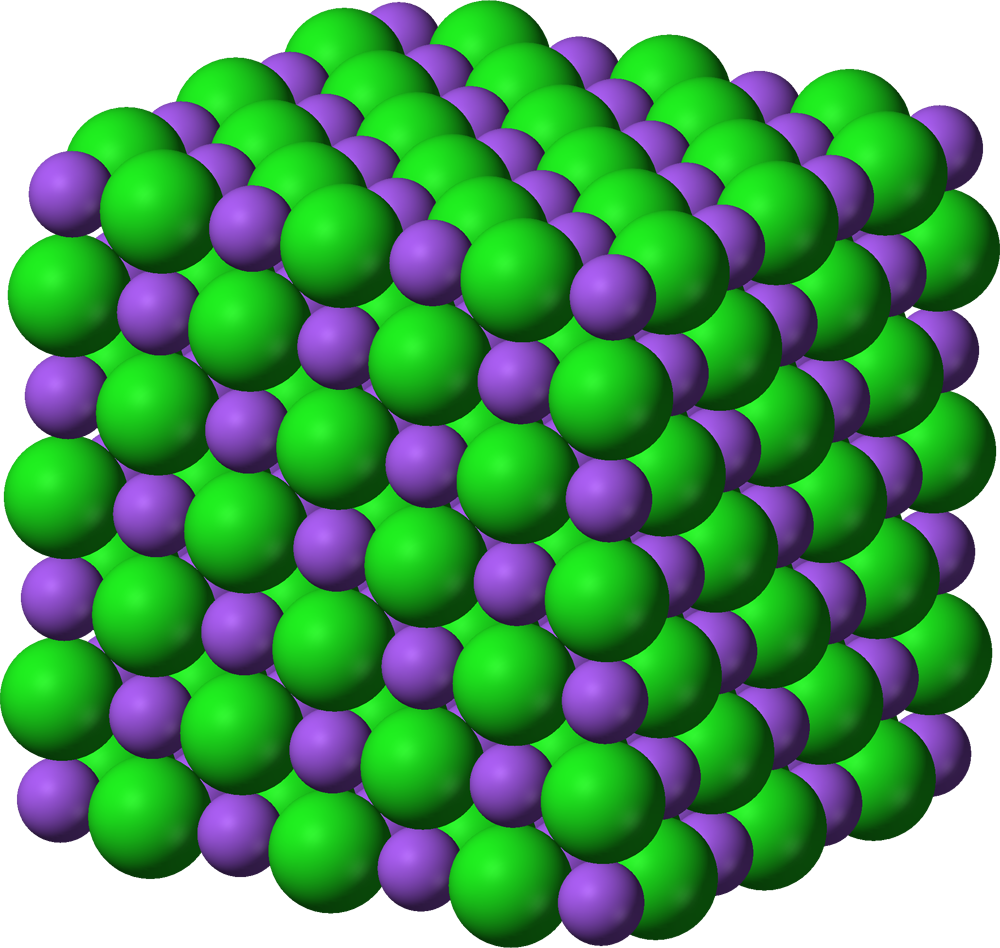
\includegraphics[width=4cm]{Sodium-chloride-3D-ionic.png}
\end{center}
includes the translations of space that move each green chlorine atom and purple natrium atom to its neighbor, up, down, left, right, forward or back, and mirror reflections around the coordinate planes through the origin, where we put the origin in the middle of any one of these atoms, and also the transformations given by permuting the order of the variables \(x,y,z\) of each coordinate axis.
\end{example}
\begin{example}
Every \(2 \times 2\) matrix 
\[
A=
\begin{pmatrix}
a & b \\
c & d
\end{pmatrix}
\]
(with entries from any chosen field) determines a \emph{linear transformation}\define{transformation!linear}\define{linear transformation}:
\[
\begin{pmatrix}
x \\
y
\end{pmatrix}
\mapsto
A
\begin{pmatrix}
x \\
y
\end{pmatrix}
=
\begin{pmatrix}
a & b \\
c & d
\end{pmatrix}
\begin{pmatrix}
x \\
y
\end{pmatrix}
=
\begin{pmatrix}
ax + by \\
cx + dy
\end{pmatrix}
\]
of the plane.
Similarly, a square matrix \(A\), say \(n \times n\), determines a linear transformation of \(n\)-dimensional Euclidean space.
A linear transformation is a bijection just when the associated matrix \(A\) is invertible, i.e. just when \(A\) has nonzero determinant.\SubIndex{determinant}
The invertible \(n \times n\) matrices form a transformation group \(G\), of linear transformations of \(n\)-dimensional Euclidean space.
\end{example}



\section{Permutations}
A transformation which is a bijection is also called a \emph{permutation}, especially when it transforms a finite set.
\begin{example}
Take \(X\) to be the set of numbers \(\set{1,2,3,4}\).
The \emph{symmetric group}\define{symmetric group} on 4 letters is the group \(G\) of all permutations of \(X\).
The terminology ``on 4 letters'' reminds us that we could just as well have taken \(X=\set{a,b,c,d}\) to consist of any 4 distinct elements, and then we would get essentially the same story, just relabelling.
It is convenient notation to write a permutation of finite sets as, for example,
\[
\begin{pmatrix}
1 & 2 & 3 & 4 \\
2 & 3 & 1 & 4
\end{pmatrix}
\]
to mean the map \(f\) so that \(f(1)=2\), \(f(2)=3\), \(f(3)=1\) and \(f(4)=4\), i.e. reading down from the top row as the input to \(f\) to the entry underneath as the output of \(f\).
It is often understood that the first row is just \(1234\) or some such, so we can just write down the second row: \(2314\), to display the permutation.
\end{example}

\begin{problem}{groups:compose.permutation}
What is are the permutations \(g \circ f\) and \(f \circ g\) where \(g\) is \(2314\) and \(f\) is \(3124\)?
\end{problem}

\begin{problem}{groups:tetrahedron}
A \emph{regular tetrahedron}\define{tetrahedron} is a pyramid with triangular base, all of whose sides are equilateral triangles.
Prove that the symmetry group of the regular tetrahedron is the symmetric group on 4 letters.
\end{problem}
\begin{answer}{groups:tetrahedron}
We can simply permutate the vertices in any way at all by symmetries, as we can rotate any one vertex to any other, and then fixing that vertex, the symmetries of the opposite faceare arbitrary symmetries of an equilateral triangle, so carry out any permutation of its vertices.
\end{answer}

Another notation for permutations: the \emph{cycle}\define{cycle} \((1 3 4 2)\) means the permutation that takes \(1\) to \(3\), \(3\) to \(4\), \(4\) to \(2\) and \(2\) to \(1\), reading from left to right.
More generally, the cycle \((a_1 a_2 \dots a_k)\) is the permutation taking \(a_1\) to \(a_2\), \(a_2\) to \(a_3\), and so on, and taking \(a_k\) to \(a_1\).
So \((2 3 1 4)\) takes \(3\) to \(1\).
By definition, if we have a number \(x\) which is not among these various \(a_1, a_2, \dots, a_k\), then the cycle \((a_1 a_2 \dots a_k)\) fixes the number \(x\):
\((2 3 5 4)\) takes \(1\) to \(1\).
Two cycles \((a_1 a_2 \dots a_k)\) and \((b_1 b_2 \dots b_{\ell})\) are \emph{disjoint}\define{cycle!disjoint} if none of the \(a_i\) occur among the \(b_j\) and vice versa.
So 
\[
(1 4 5 2) \text{ is disjoint from } (3 6),
\]
but
\[
(1 3 5 2) \text{ is not disjoint from } (3 6)
\]
since they both have \(3\) in them.
We can write the identity permutation as \(()\).
Note that any cycle of length 1 is also the identity transformation: \((2)=(1)=()\), since \((2)\) takes \(2\) to \(2\), and fixes everything else.
If two permutations \(f\) and \(g\) can be expressed as disjoint cycles, then \(fg=gf\), since each fixes all of the letters moved by the other.

\begin{problem}{permutations:disjointify}
Write \((123)(234)(543)\) as (a) a permutation in our first notation and (b) as  a product of disjoint cycles.
\end{problem}
\begin{answer}{permutations:disjointify}
Apply each cycle in succession to \(1\): \((543)1=1\), \((234)1=1\), \((123)1=2\). So \((123)(234)(543)1=2\).
Similarly apply them to \(2\): \((543)2=2\), \((234)2=3\), \((123)3=1\). So \((123)(234)(543)2=1\).
Continue in this way to find (a) \((123)(234)(543)=21543\).
Clearly this takes \(1 \to 2 \to 1\) and \(3 \to 5 \to 3\) and \(4 \to 4\), so (b) as a product of disjoint cycles
\((123)(234)(543)=(12)(35)\).
\end{answer}

Sage knows how to multiply cycles:
\begin{sageblock}
G = SymmetricGroup(5)
sigma = G("(1,3) (2,5,4)")
rho = G([(2,4), (1,5)])
rho^(-1) * sigma * rho
\end{sageblock}
prints \(\sage{rho^(-1) * sigma * rho}\).

\begin{theorem}
Every permutation of the elements of a finite set is expressed as a product of disjoint cycles, uniquely except for the order in which we write down the cycles, which can be arbitrary.
\end{theorem}
\begin{proof}
Suppose our finite set is \(1,2,\dots,n\); write these down in order in a list.
Pick a number and see what the permutation takes it to, and what it takes that number to, and so on, until eventually you return to the number you started at: a cycle.
Cross out all of those numbers from the list, and start again.
\end{proof}

For example, in cycle notation
\[
\begin{pmatrix}
1 & 2 & 3 & 4 \\
2 & 3 & 1 & 4
\end{pmatrix}
=(1 2 3)
\]
and
\[
\begin{pmatrix}
1 & 2 & 3 & 4 & 5 \\
3 & 4 & 1 & 5 & 2 
\end{pmatrix}
=(1 3)(2 4 5).
\]
\begin{problem}{permutations:cycle.product}
What is the product of cycles \((1234)(1423)(324)\) as a product of disjoint cycles?
Explain how you find your answer.
\end{problem}
\begin{answer}{permutations:cycle.product}
\((234)\): 
\begin{align*}
1 &\to 4 \to 1, \\
2 &\to 4 \to 2 \to 3, \\
3 &\to 2 \to 3 \to 4, \\
4 &\to 3 \to 1 \to 2.
\end{align*}
\end{answer}
\begin{problem}{permutations:cube}
Let \(G\) be the collection of all rotations of a cube.
How many rotations lie in \(G\)?
How does each decompose into a product of disjoint cycles acting on the faces of the cube?
\end{problem}
\begin{answer}{permutations:cube}
Indicate cycle lengths in a permutation by drawing boxes, a row of them to indicate a cycle of that length, arranged successively shorter: the \emph{Young diagram}\define{Young diagram} of a permutation.
For example, 
\[
\yng(4,3^2,2)
\]
indicates a permutation which has cycles of lengths \(4,3,3,2\).
The group \(G\) of rotations of a cube moves any vertex to any other (8 in all), and rotates a vertex around taking any edge at that vertex to any other (3 in all), but once we fix a vertex and edge, we fix everything, so the group has exactly \(8\cdot 3=24\) elements.
Every rotation is a rotation around an axis, through the centre of the cube.
It is determined completely by how it acts on the centres of the faces, as they contain a basis of vectors.
The identity \(1\) fixes every face, so has \(6\) cycles (all of length 1) as permutation of the faces.
A rotation of angle \(\pi\) around an axis through the center of a face fixes two faces and permutes two others, so a pair of disjoint cycles of length 2; there are 3 such, as there are three choices of axis.
A rotation of angle \(\pi\) around an axis through the center of an edge permutes three pairs of faces, so a triple of disjoint cycles of length 2; there are 6 such rotations.
An element of order 3 is a rotation around an axis through two opposite corners: it is a cycle of order 3 on the three faces touching one corner, and also of order 3 on the opposite three faces touching the opposite corner.
There are 4 choices of a pair of opposite corners, and then 2 directions of rotation, so 8 such rotations.
An element of order 4 is a rotation by angle \(\pi/2\), so around some axis through two opposite faces, giving one cycle of length 4; there are 3 choices of axis, but we can point the axis in either direction, so 6 such rotations.
We can sum the various permutations of the faces of cube arising from rotations as:
\[
\yng(1^6)+3\yng(2^2,1^2)+6\yng(2^3)+8\yng(3^2)+6\yng(4,1,1)
\]
\end{answer}
\begin{problem}{groups:count.perms}
Prove that any set with \(n\) elements has \(n!\) permutations, in several ways: by counting 
\begin{enumerate}
\item how many places to move \(1\) to, and then how many places there are left to move \(2\) to, and so on,
\item the number of places to stick object \(n\) in between the elements of any given permutation \(a_1 a_2 \dots a_{n-1}\) of the numbers \(1,2,\dots,n-1\), say as \(n a_1 a_2 \dots a_{n-1}\) or \(a_1 n a_2 \dots a_{n-1}\) or \(a_1 a_2 n \dots a_{n-1}\) and so on, for example: given the permutation \(312\) of the numbers \(123\), we can put \(4\) in there as
\[
4312, 3412, 3142, \text{ or } 3124.
\]
\item the number of ways to put at the end of a given permutation \(a_1 a_2 \dots a_{n-1}\) some number \(b\) from among 
\[
b=\frac{1}{2}, 1+\frac{1}{2}, \dots, n-\frac{1}{2},
\]
for example into the permutation \(312\) we stick
\[
312\frac{1}{2}, \quad \text{ or }
312\frac{3}{2}, \quad \text{ or }
312\frac{5}{2}, \quad \text{ or }
312\frac{7}{2}
\]
and then replace the numbers in the list by integers from \(1,2,\dots,n\), but in the same order:
\[
4231, 4132, 4123, \text{ or } 3124.
\]
\item
the possible disjoint cycles.
\end{enumerate}
\end{problem}
\begin{problem}{groups:symmetric.conjugacy.1}
Suppose that \(g\) is a permutation written as a product of disjoint cycles, say \(g=(1487)(235)\) as a permutation of 8 letters.
Take any permutation \(h\) of 8 letters.
Prove that 
\[
hgh^{-1}=(h(1)h(4)h(8)h(7))(h(2)h(3)h(5)).
\]
\end{problem}
\begin{answer}{groups:symmetric.conjugacy.1}
In general, if 
\[
g=\dots (a_1 a_2 \dots a_k) \dots
\]
where the \(\dots\) indicate other cycles, in a product of disjoint cycles, then \(hgh^{-1}\), when applied to \(h(a_i)\) gives
\begin{align*}
(hgh^{-1})(h(a_1))
&=
hgh^{-1}h(a_1),
\\
&=
hg(h^{-1}h)(a_1),
\\
&=
hg(a_1),
\\
&=
h(a_{2}),
\end{align*}
and so on: \(hgh^{-1}\) takes \(h(a_i)\) to \(h(a_{i+1})\) and takes \(h(a_n)\) to \(h(a_1)\).
If \(g\) is a product of cycles, the same thing works applied one at a time.
\end{answer}
\begin{problem}{groups:symmetric.conjugacy}
Prove that there is an element \(g\) of the symmetric group on 7 letters so that \((147)(23)\) and \((235)(14)\) are conjugate, i.e. \((235)(14)=g(147)(23)g^{-1}\).
More generally, prove that two elements of the symmetric group on \(n\) letters are conjugate just when, when we write them as products of disjoint cycles, the numbers of cycles of each length are the same. 
\end{problem}
\begin{answer}{groups:symmetric.conjugacy}
Start with just one cycle, say \((a_1a_2\dots a_k)\) and one cycle \((b_1b_2\dots b_k\).
Then let \(ga_1\defeq b_1\), \dots, \(ga_k\defeq b_k\), and let \(gx\defeq x\) for \(x\) not among \(a_1,\dots,a_k\).
Let's check that \((b_1\dots b_k)=g(a_1 \dots a_k)g^{-1}\).
The left hand side acts on \(b_1\) by moving it to \(b_2\), and so on.
The right hand side takes \(b_1\), applies \(g^{-1}\) to it, so gives \(a_1\), then moves \(a_1\) to \(a_2\), and then applies \(g\) to that, giving \(b_2\), and so on.
Now for two disjoint cycles, say 
\[
g_1 = (a_1 a_2 \dots a_k)(\alpha_1 \alpha_2 \dots \alpha_{\ell})
\]
and
\[
g_2 = (b_1 b_2 \dots b_k)(\beta_1 \beta_2 \dots \beta_{\ell}),
\]
let \(ga_i \defeq b_1\) and \(g\alpha_i\defeq \beta_i\) and \(gx=x\) for any other \(x\).
Again check that \(g_2=gg_1g^{-1}\).
Proceed by induction.
\end{answer}
A \emph{transposition}\define{transposition} is a 2-element cycle.
Every cycle has an obvious decomposition as a product of transpositions: \((1234)=(12)(23)(34)\), and so on: 
\begin{problem}{permutations:cycle.as.transpositions}
Prove that \((123\dots n)=(12)(23)(34)\dots(n-1 \ n)\).
\end{problem}
Hence we can break any permutation into an obvious product of transpositions.
\begin{problem}{permutations:transposition.product}
Write the permutation \((17)\) as a product of transpositions of neighboring integers.
\end{problem}
\begin{answer}{permutations:transposition.product}
\((12)(23)(34)(45)(56)(67)(56)(45)(34)(23)(12)\)
\end{answer}
Given a polynomial \(b(t)\) in variables \(t_1,t_2,\dots,t_n\), and a permutation \(p\) of \(n\) letters, we define \(pb(t)\) by the equation
\[
pb(t_1,\dots,t_n)=b(t_{q(1)},\dots,t_{q(n)}),
\]
where \(q\) is the inverse permutation to \(p\).
\begin{example}
If \(p=2314\) then \(q=3124\). If
\[
b(t_1,t_2,t_3,t_4)=t_1^6+8t_2t_4+t_3^9,
\]
then
\[
pb(t_1,t_2,t_1,t_4)=t_3^6+8t_1t_4+t_2^9.
\]
\end{example}
\begin{problem}{groups:compose.poly}
If \(p,r\) are permutations on \(n\) letters prove that \(r(pb)=(rp)b\) for any polynomial \(b\) in \(n\) variables.
\end{problem}
\begin{answer}{groups:compose.poly}
Let \(q\defeq p^{-1}\) and \(s\defeq r^{-1}\), so
\begin{align*}
(r(pb))(t_1,\dots,t_n)
&=
pb(t_{s(1)},\dots,t_{s(n)}),
\\
&=
b(t_{q(s(1))},\dots,t_{q(s(n))}),
\\
&=
b(t_{q \circ s(1))},\dots,t_{q \circ s(n))}),
\\
&=
(q \circ s)^{-1}b(t_1,\dots,t_n),
\\
&=
(s^{-1} \circ q^{-1})b(t_1,\dots,t_n),
\\
&=
(rp)b(t_1,\dots,t_n).
\end{align*}
\end{answer}
The \emph{sign}\define{sign!permutation}\define{permutation!sign} of a permutation \(p\), denoted \((-1)^p\), is \((-1)^t\) where \(t\) is the number of transpositions in some expression of \(p\) as a product of transpositions of neighboring integers.
\begin{lemma}\label{lemma:sign.of.permutation}
The map taking a permutation \(p\) to its sign, denoted \((-1)^p\), is well defined and satisfies \((-1)^{pq}=(-1)^p(-1)^q\) for any two permutations \(p,q\) of the same number of letters.
Moreover \((-1)^p=(-1)^t\) if \(p\) can be written as as product of \(t\) transpositions.
\end{lemma}
\begin{proof}
Consider the polynomial
\[
b(t_1,\dots,t_n)=(t_1-t_2)(t_1-t_3)\dots(t_{n-1}-t_n)=\prod_{i<j}(t_i - t_j).
\]
Then \(pb(t)\) has various \(t_i-t_j\) factors multiplied together, with \(i \ne j\), in every possible pairing of \(i,j\) or \(j,i\).
So \(pb(t)=\pm b(t)\).
Write this \(\pm\) as \((-1)^p\).

Suppose that \(p\) is the transposition \((i \ \ i+1)\).
Then \(p\) changes \(t_i-t_{i+1}\) into \(t_{i+1}-t_i=-(t_i-t_{i+1})\), one sign change.
Otherwise, \(p\) leaves everything in \(b(t)\) as it is except swapping \(t_i-t_j\) and \(t_{i+1}-t_j\) for \(j \ge i+2\), and swapping \(t_j-t_i\) and \(t_j-t_{i+1}\) for \(j \le i-1\).
So finally, only one sign change: \(pb(t)=-b(t)\), so \((-1)^p=-1\).

If \(p,q\) are any two permutations of \(n\) letters, then \((-1)^p(-1)^qb=p(qb)=(pq)b=(-1)^{pq}b\).
Therefore, for any \(i\) and \(j\), if we write
\[
(i \ \ i+1)=(i+1 \ \ j)(i \ \ j)(i+1 \ \ j),
\]
then \((-1)^{(ij)}=(-1)^{(i \ \ i+1)}=-1\).
\end{proof}
\begin{problem}{permutations:transposition}
Prove that the sign of any transposition is \(-1\) by writing it as a product number of transpositions of neighboring integers.
\end{problem}
\begin{answer}{permutations:transposition}
We can transpose \(i\) and \(i+1\) as \((i \ \ i+1)\).
We can transpose \(i\) and \(i+2\), as a product \((i \ \ i+1)(i+1 \ \ i+2)(i \ \ i+1)\).
Similarly, we can write any transposition as a product of an odd number of transpositions of neighboring integers: if \(i<j\),
\[
(i \ \ j)=(i \ \ i+1)(i+1 \ \ i+2)\dots(j-2 \ \ j-1)(j-1 \ \ j)\dots(i+1 \ \ i+2)(i \ \ i+1).
\]
\end{answer}
\begin{problem}{permutions:rationals}
Prove that, over any field, any symmetric rational function (i.e. permutation invariant) has an expression \(b(e_1,\dots,e_n)/c(e_1,\dots,e_n)\) as a ratio of polynomials with no common nonconstant factor, expressed in the elementary symmetric polynomials, unique up to rescaling numerator and denominator by the same nonzero constant.
\end{problem}
\begin{answer}{permutions:rationals}
If there were two such, cross multiply and apply unique factorisation of polynomials (theorem~\vref{theorem:ufd}).
To see that there is one such, write out the function as \(p(x_1,\dots,x_n)/q(x_1,\dots,x_n)\).
Apply a permutation of the variables, and the solution of problem~\vref{problem:factoring:rationals}, to see that each permutation alters the numerator by a nonzero constant multiple, and the denominator by the same multiple.
Swapping two variables gives some multiple, and repeating that swap gives the same multiple squared, but returns to the original order of the variables.
So any swap either changes sign or leaves both numerator and denominator alone.
Multiple the numerator and denominator by the function \(\prod_{i<j}(t_i - t_j)\) to ensure that the don't change when we transpose, and so they don't change under any permutation.
Apply theorem~\vref{theorem:symmetric.polynomials.algebra}.
\end{answer}
\begin{problem}{permutations:det}
Starting from your favourite definition of determinant of a square matrix, prove that for any square matrix \(A\), say of size \(n \times n\), with coefficients in any field,
\[
\det A = \sum_p (-1)^p A_{1p(1)}A_{2p(2)} \dots A_{np(n)},
\]
where the sum is over all permutations \(p\) of \(1,2,\dots,n\).
\end{problem}
The group of even permutations of \(n\) letters is the \emph{alternating group}.
\begin{problem}{permutations:alt.4}
Write out the elements of the alternating group on \(4\) letters.
\end{problem}
\begin{problem}{permutations:alt}
Prove that the alternating group on \(n\) letters contains \(n!/2\) elements.
\end{problem}
\begin{problem}{permutations:15}
The \(15\)-puzzle is a \(4 \times 4\) square containing with \(15\) slideable tiles (each a \(1 \times 1\) square), so one square is vacant (i.e. has no tile in it):
\begin{center}
\documentclass[tikz]{standalone}
\begin{document}
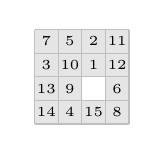
\begin{tikzpicture}[scale=.3]
\fill[gray!20] (0,0) rectangle (4,4);
\fill[white] (2,1) rectangle (3,2);
\draw[gray!50] (0,0) grid (4,4);
\node at (.5,3.5) {\tiny{7}};
\node at (1.5,3.5) {\tiny{5}};
\node at (2.5,3.5) {\tiny{2}};
\node at (3.5,3.5) {\tiny{11}};
\node at (.5,2.5) {\tiny{3}};
\node at (1.5,2.5) {\tiny{10}};
\node at (2.5,2.5) {\tiny{1}};
\node at (3.5,2.5) {\tiny{12}};
\node at (.5,1.5) {\tiny{13}};
\node at (1.5,1.5) {\tiny{9}};
%\node at (2.5,1.5) {\tiny{1}};
\node at (3.5,1.5) {\tiny{6}};
\node at (.5,.5) {\tiny{14}};
\node at (1.5,.5) {\tiny{4}};
\node at (2.5,.5) {\tiny{15}};
\node at (3.5,.5) {\tiny{8}};
\end{tikzpicture}
\end{document}
\end{center}
Each tile has a number on it, from 1 to 15.
We solve the puzzle by sliding the squares around until they lie in order by number, with the vacant square last:
\begin{center}
\documentclass[tikz]{standalone}
\begin{document}
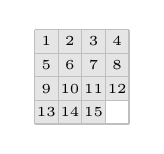
\begin{tikzpicture}[scale=.3]
\fill[gray!20] (0,0) rectangle (4,4);
\fill[white] (3,0) rectangle (4,1);
\draw[gray!50] (0,0) grid (4,4);
\node at (.5,3.5) {\tiny{1}};
\node at (1.5,3.5) {\tiny{2}};
\node at (2.5,3.5) {\tiny{3}};
\node at (3.5,3.5) {\tiny{4}};
\node at (.5,2.5) {\tiny{5}};
\node at (1.5,2.5) {\tiny{6}};
\node at (2.5,2.5) {\tiny{7}};
\node at (3.5,2.5) {\tiny{8}};
\node at (.5,1.5) {\tiny{9}};
\node at (1.5,1.5) {\tiny{10}};
\node at (2.5,1.5) {\tiny{11}};
\node at (3.5,1.5) {\tiny{12}};
\node at (.5,.5) {\tiny{13}};
\node at (1.5,.5) {\tiny{14}};
\node at (2.5,.5) {\tiny{15}};
%\node at (3.5,.5) {\tiny{8}};
\end{tikzpicture}
\end{document}
\end{center}
Prove that if the 15-puzzle starts in this order:
\begin{center}
\documentclass[tikz]{standalone}
\begin{document}
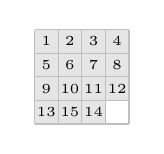
\begin{tikzpicture}[scale=.3]
\fill[gray!20] (0,0) rectangle (4,4);
\fill[white] (3,0) rectangle (4,1);
\draw[gray!50] (0,0) grid (4,4);
\node at (.5,3.5) {\tiny{1}};
\node at (1.5,3.5) {\tiny{2}};
\node at (2.5,3.5) {\tiny{3}};
\node at (3.5,3.5) {\tiny{4}};
\node at (.5,2.5) {\tiny{5}};
\node at (1.5,2.5) {\tiny{6}};
\node at (2.5,2.5) {\tiny{7}};
\node at (3.5,2.5) {\tiny{8}};
\node at (.5,1.5) {\tiny{9}};
\node at (1.5,1.5) {\tiny{10}};
\node at (2.5,1.5) {\tiny{11}};
\node at (3.5,1.5) {\tiny{12}};
\node at (.5,.5) {\tiny{13}};
\node at (1.5,.5) {\tiny{15}};
\node at (2.5,.5) {\tiny{14}};
%\node at (3.5,.5) {\tiny{8}};
\end{tikzpicture}
\end{document}
\end{center}
it is not solvable.
Hint: associate to each permutation (of tiles and vacant square) a number \(x=0\) or \(1\), depending on whether the permutation of the order of the tiles (ignoring the vacant spot) is even or odd, and a number \(y=0\) or \(1\) given by the row of the vacant spot, modulo \(2\).
Let \(z=x+y\) modulo 2.
\end{problem}
\begin{answer}{permutations:15}
If we make a move by sliding a tile left or right, we don't change \(x\) or \(y\), so \(z\) is the same.
If we make a move by sliding a tile up or down, we change \(y\) and also carry out a cycle in the order of the tiles.
If that tile is in the first column, we are making a cycle of length 4:
\begin{center}
\documentclass[tikz]{standalone}
\begin{document}
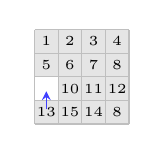
\begin{tikzpicture}[scale=.3]
\fill[gray!20] (0,0) rectangle (4,4);
\fill[white] (0,1) rectangle (1,2);
\draw[gray!50] (0,0) grid (4,4);
\node at (.5,3.5) {\tiny{1}};
\node at (1.5,3.5) {\tiny{2}};
\node at (2.5,3.5) {\tiny{3}};
\node at (3.5,3.5) {\tiny{4}};
\node at (.5,2.5) {\tiny{5}};
\node at (1.5,2.5) {\tiny{6}};
\node at (2.5,2.5) {\tiny{7}};
\node at (3.5,2.5) {\tiny{8}};
%\node at (.5,1.5) {\tiny{9}};
\node at (1.5,1.5) {\tiny{10}};
\node at (2.5,1.5) {\tiny{11}};
\node at (3.5,1.5) {\tiny{12}};
\node at (.5,.5) {\tiny{13}};
\node at (1.5,.5) {\tiny{15}};
\node at (2.5,.5) {\tiny{14}};
\node at (3.5,.5) {\tiny{8}};
\draw[shorten >=1pt,shorten <=1pt,blue!75,-stealth] (.5,.5) -- (.5,1.5);
\end{tikzpicture}
\end{document}
\end{center}
and the same for any other column, since we have one less square above and one more below.
So the value of \(x\) always changes.
So \(z\) stays the same.
The initial picture:
\begin{center}
\documentclass[tikz]{standalone}
\begin{document}
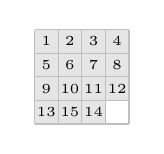
\begin{tikzpicture}[scale=.3]
\fill[gray!20] (0,0) rectangle (4,4);
\fill[white] (3,0) rectangle (4,1);
\draw[gray!50] (0,0) grid (4,4);
\node at (.5,3.5) {\tiny{1}};
\node at (1.5,3.5) {\tiny{2}};
\node at (2.5,3.5) {\tiny{3}};
\node at (3.5,3.5) {\tiny{4}};
\node at (.5,2.5) {\tiny{5}};
\node at (1.5,2.5) {\tiny{6}};
\node at (2.5,2.5) {\tiny{7}};
\node at (3.5,2.5) {\tiny{8}};
\node at (.5,1.5) {\tiny{9}};
\node at (1.5,1.5) {\tiny{10}};
\node at (2.5,1.5) {\tiny{11}};
\node at (3.5,1.5) {\tiny{12}};
\node at (.5,.5) {\tiny{13}};
\node at (1.5,.5) {\tiny{15}};
\node at (2.5,.5) {\tiny{14}};
%\node at (3.5,.5) {\tiny{8}};
\end{tikzpicture}
\end{document}
\end{center}
differs from the final one:
\begin{center}
\documentclass[tikz]{standalone}
\begin{document}
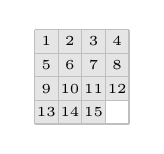
\begin{tikzpicture}[scale=.3]
\fill[gray!20] (0,0) rectangle (4,4);
\fill[white] (3,0) rectangle (4,1);
\draw[gray!50] (0,0) grid (4,4);
\node at (.5,3.5) {\tiny{1}};
\node at (1.5,3.5) {\tiny{2}};
\node at (2.5,3.5) {\tiny{3}};
\node at (3.5,3.5) {\tiny{4}};
\node at (.5,2.5) {\tiny{5}};
\node at (1.5,2.5) {\tiny{6}};
\node at (2.5,2.5) {\tiny{7}};
\node at (3.5,2.5) {\tiny{8}};
\node at (.5,1.5) {\tiny{9}};
\node at (1.5,1.5) {\tiny{10}};
\node at (2.5,1.5) {\tiny{11}};
\node at (3.5,1.5) {\tiny{12}};
\node at (.5,.5) {\tiny{13}};
\node at (1.5,.5) {\tiny{14}};
\node at (2.5,.5) {\tiny{15}};
%\node at (3.5,.5) {\tiny{8}};
\end{tikzpicture}
\end{document}
\end{center}
by a single transposition, with no row swap, so different value of \(z\).
\end{answer}

\section{Sage}
Sage knows all of the permutations of small symmetric groups, and will print them out for you in cycle notation:
\begin{sageblock}
H = DihedralGroup(6)
H.list()
\end{sageblock}
yields
\[
\begin{array}{lll}
               , & (1,6)(2,5)(3,4), & (1,2,3,4,5,6), \\ 
     (1,5)(2,4), & (2,6)(3,5),      & (1,3,5)(2,4,6), \\ 
(1,4)(2,3)(5,6), & (1,6,5,4,3,2),   & (1,4)(2,5)(3,6), \\ 
(1,2)(3,6)(4,5), & (1,5,3)(2,6,4),  & (1,3)(4,6)
\end{array}
\]
where the identity element is the blank space at the start.
